% chapter 2
\chapter{Context}
Before we proceed the actual content of the study, it is useful to introduce some concepts that will help the reader
to understand the ideas discussed in this project. In this section, we will explain the basics of
linear and integer programming and basic algorithms used for solving them, followed by explanation on why
constraints programming is suitable for solving LP problems and some background information on the chosen LP tools. Last but not least,
we also explain some terminologies on graph theory that will be used when dealing with vehicle routing problem.

\section{Linear Programming}
Linear programming (LP) is a mathematical method to obtain the optimal solution of a function in a linear system under set of constraints
imposed on its variables. It is a method commonly used in solving combinatorial optimisation problems in applied mathematics and operations research.
A problem is considered a linear program when all of its mathematical relationship are linear \cite{APMBradley}.
The word 'programming' is not to be confused with the term used in computer science,
in which concerns with creating instructions for computers to execute. A linear
program consists of three entities \cite{LPChvatal,ILPCoursera}:
\begin{enumerate}
\item \textbf{Decision variables} - These are the entities that can be controlled by the decision maker.
\item \textbf{Objective function} - This is the function that, given the optimal input, outputs the optimal value.
In most cases, it is to find the minimum or the maximum value.
\item \textbf{Variable constraints} - These are the restrictions that are imposed on the decision variables. There are two types
of constraints: hard and soft. Hard constraints are constraints cannot be violated at all cost, whereas soft constraints may be
violated, but should be observed wherever possible.
\end{enumerate}

To fully understand LP, it is best to look at an example: Bob is competing in
an eating contest that lasts one hour where the objective is to accumulate as much points as possible by eating a combination of hotdogs and burgers.
For each burger and hotdog that Bob eats, he will get 5 and 4 points respectively. It takes him 3 minutes to finish a burger and
2 minutes to finish a hotdog. Bob can consume 25 food items before his appetite reaches its limit.

Based on the scenario above, we can model this problem in the form of a linear program by following these steps:
\begin{itemize}
\item \textbf{Step 1}: Identify the decision variables. Let \(x\) be the number of hotdogs and \(y\) be the number
of burgers eaten by Bob.
\item \textbf{Step 2}: Determine the objective function. In this scenario, we want to determine the highest possible
points that Bob can achieve in the competition. This can be represented by the equation \(z = 4x + 5y\), where
z is the value of the points accumulated in the competition and the coefficients of the variables represent the points achieved by eating respective
food items.
\item \textbf{Step 3}: Determine the constraints. There are 3 constraints in these problem. Firstly, The amount of
food eaten by bob has to be under 60 minutes. This can be represented by the equation \(2x + 3y \leq 60\). Secondly,
Bob's appetite has a limit of 25 food items, which can be modelled with the equation \(x + y \leq 25\). Lastly,
the number of respective food eaten has to be greater than or equal to 0.
\end{itemize}
Putting them together, we have the following linear program:
\[
  \begin{array}{r@{}r@{}l}
    \text{Maximise z =} \quad &{}4x + 5y \\[\jot]
    \text{Subject to}\qquad &{} 2x +   3y &{} \leq 60 \\
    \qquad &{} x +   \phantom{2}y &{} \leq 25 \\
    \qquad &{} x ,   \phantom{2}y &{} \geq 0 \\
  \end{array}
\]
There are two types of solution that can be produced. A feasible solution is a set of variables that satisfies the constraints
of a linear program. An example of a feasible solution for the above solution would be \(x = 25\) and \(y=0\), which yields 100 points.
The goal of the linear program is to achieve optimal solution of the objective function \cite{LPChvatal}. The optimal solution is the best feasible solutions.
For the problem above, the optimal solution is 110 points, which is produced when \(x = 15\) and \(y = 10\). The feasible solutions
are bound within the feasible region marked in green as shown in Figure 2.1. The red region is the infeasible region, where any point that falls within it will not satisfy the
constraints of the linear program. The dimensions of the graph is determined by the number of variables the linear program has.
So, a linear program with three variables can only be described with three dimensional graph.

There are three types of outcomes \cite{LPChvatal,ILPCoursera} in a linear program and they are determined by the
its feasible region. The three outcomes are:
\begin{itemize}
\item \textbf{Outcome 1} : The feasible region is unbounded, thus the objective function is infinity.
\item \textbf{Outcome 2} : The feasible region is empty, this is usually because the constraints on the variables contradict each other.
\item \textbf{Outcome 3} : The feasible region is bounded. In this case, an optimal solution exists.
\end{itemize}

\begin{figure}[!ht]
  \centering
    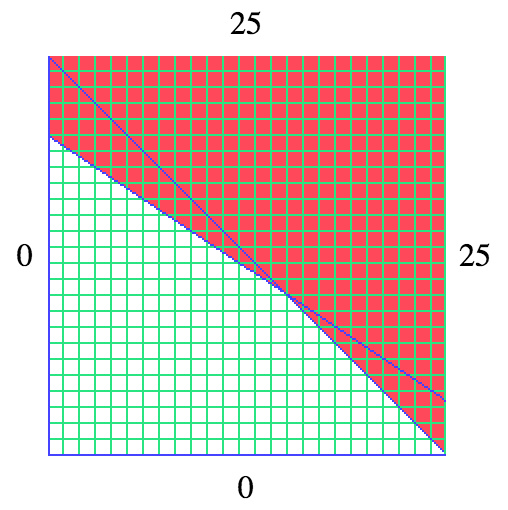
\includegraphics[width=0.5\textwidth]{example-graph.png}
    \caption{Graphical representation of the linear program example. Figure taken from \url{http://www.zweigmedia.com/}\cite{zweigmedia}}
\end{figure}

To find the optimal solution, we use the simplex method \cite{LPChvatal, LPVanderbei}. The simplex method starts off by selecting a point in a graph.
Then it moves to a different point of the graph. On each move, it will make sure that the point yield higher
objective value. If no higher objective value is found, then that point would be the
optimal solution. This method also works in higher dimensional spaces. The illustration of this algorithm is shown in figure 2.2.
For the complete explanation on the simplex method, refer to these references \cite{LPChvatal, LPVanderbei}.

\begin{figure}[!ht]
  \centering
    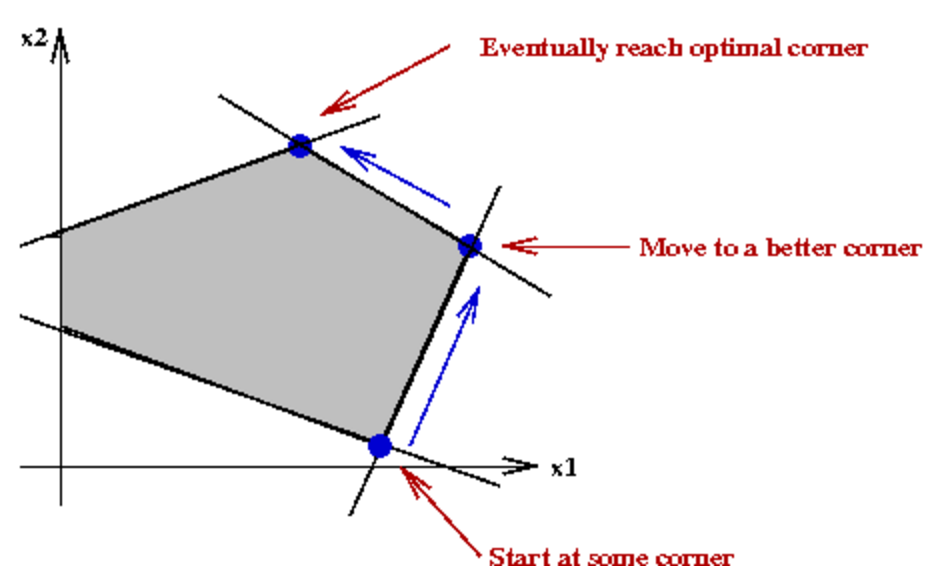
\includegraphics[width=0.8\textwidth]{simplex2.png}
    \caption{Simplex method on a linear program, taken from George Washington University \cite{seas:SM}}
    \vspace{1cm}
    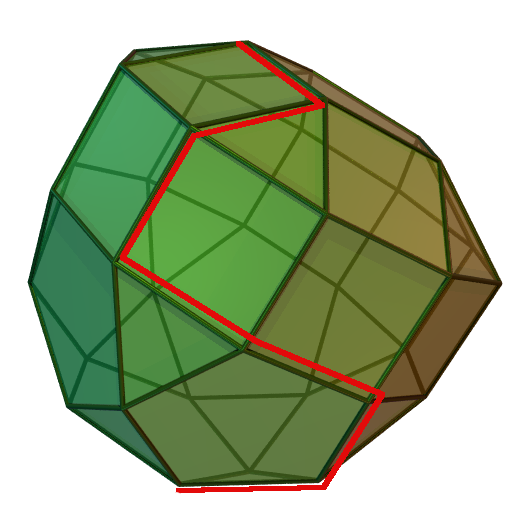
\includegraphics[width=0.5\textwidth]{simplex3d.png}
    \caption{Simplex algorithm on a three dimensional representation of a linear program, taken from Wikipedia \cite{Wiki:SPM}}
    \vspace{1cm}
\end{figure}

\section{Integer Programming}
Integer programming (IP) \cite{LPVanderbei} is a linear program that has an additional
integrality constraint of imposed on to its decision variables. This is useful in situations where the values need to be
discrete, such as the number of people or boolean values.
When this constraint is added, finding an optimal solution becomes harder. This is because the solution space is reduced to
the lattice points of feasible region. Linear programming that has both real valued and integer valued constraints on its
 decision variables is called Mixed Integer Programming (MIP) \cite{LPVanderbei}.
Also mention about IP being NP Complete and then refer to computational complexity note etc...

\begin{figure}[!ht]
  \centering
    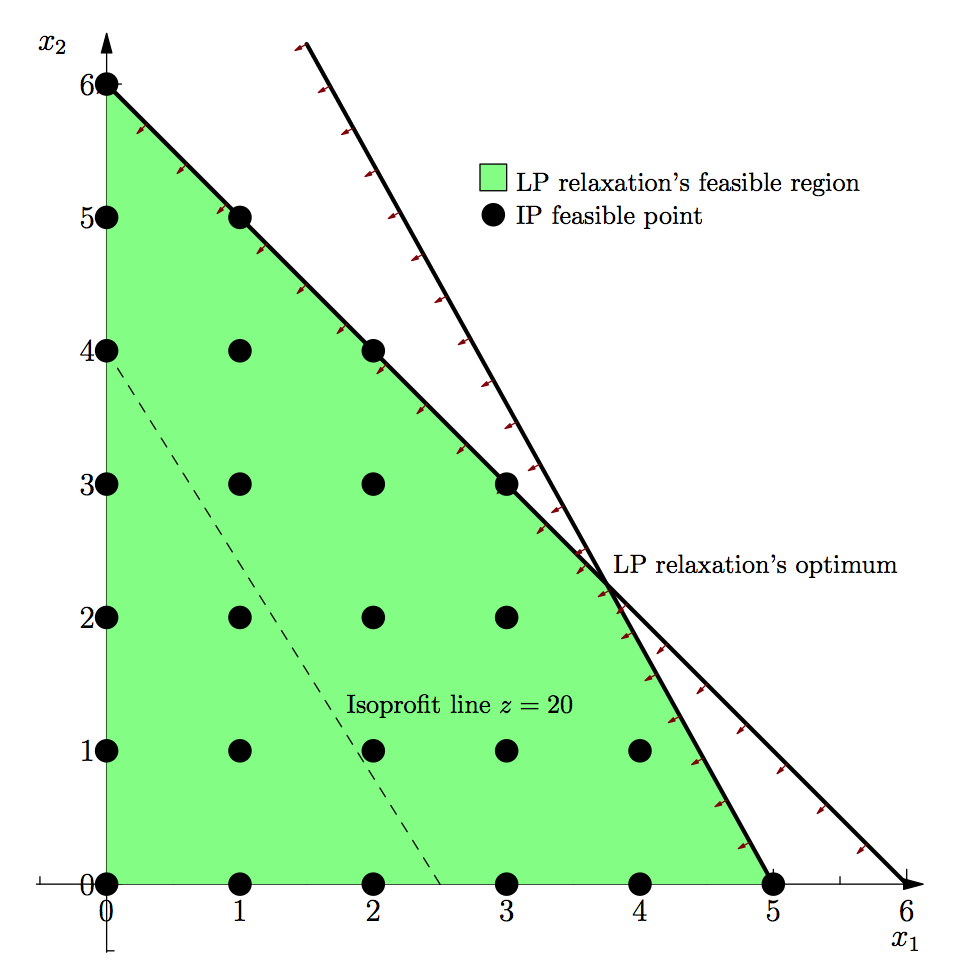
\includegraphics[width=0.7\textwidth]{ipfeasible.png}
    \caption{Feasible solutions of an integer program marked by the black dots (lattice points) bounded by the feasible region (green region), taken from
     Linear Programming: Foundations and Extensions by Robert Vanderlei \cite{Sottinen2009}}
\end{figure}

More sophisticated algorithms have been invented in order to accomodate the added complexity of IP. One of the most commonly
used algorithm that uses exact approach to finding a solution is the branch-and-bound algorithm  \cite{LPVanderbei, LPChvatal, Dastghaibifard2008}. It uses divide and
conquer approach to partition the problem into sub-problems
and then solves them recursively. LP methods such as the simplex can be used to solve the sub-problems \cite{Dastghaibifard2008}.
The 'branching' part generates a tree
that continues to expand until all valid solutions are found. The bound part compares all solutions and keeps the
most optimal one.

For the sake of clarity, we shall solve an example problem below \cite{LPVanderbei} to see how IP works:
\[
  \begin{array}{r@{}r@{}l}
    \text{Maximise} \quad &{}x_{1} + 12x_{2} \\[\jot]
    \text{subject to}\qquad &{}10x_{1} +   7x_{2} &{} \leq 40 \\
    \qquad &{} x_{1} +   \phantom{2}x_{2} &{} \leq 5 \\
    \qquad &{} x_{1} ,   \phantom{2}x_{2} &{} \in \mathbb{Z}_{>0}\\
  \end{array}
\]

These are the steps of the branch of bound algorithm as it solves the IP problem above:
\begin{itemize}
\item The 'branch' part:
    \begin{itemize}
        \item \textbf{Step 1} : We start by solving the given IP problem using standard LP method such as the simplex algorithm. Then, we pick
         real-valued decision variables as the branching variables. If there are no real-valued variables, go to step 3.
         At this point, We are at the root of the tree that is generated by this algorithm.
        \item \textbf{Step 2} : Create 2 branches for the chosen branching variable and set a new constraints to that variable in those branches
        . For example, in the children of the root node of the figure 2.5,
         we impose the constraint \(x_{1} \leq 1\) on the left side and \(x_{1} \geq 2\) on the right side of the branch.
        \item \textbf{Step 3} : This is the recursive step of the branching algorithm. We pick a branch and then solve it
        using the same method in step 1. At this point, there are 3 possible outcomes:
            \begin{enumerate}
                \item Infeasible solution: the algorithm will not continue branching from this node and picks other unexplored node
                to solve.
                \item Integral solution found : the branching will stop here, record the solution and move on to solve other unexplored node.
                \item Fractional/real solution found: branch this node and then go back to step 2.
                Exit if there are no explored nodes left.
            \end{enumerate}
    \end{itemize}
\item The 'bound' part: The algorithm will compare all solutions found and keep the most optimal one. The optimal value is set negative infinity at first
and it will be immediately replaced as soon as an integral solution is found.
 This will give the exact solution of the problem. The optimal value of this integer program is 68, where \(x_{1} = 4\) and \(x_{2} = 0\).
\end{itemize}

\vspace{0.5cm}

\begin{figure}[!ht]
  \centering
    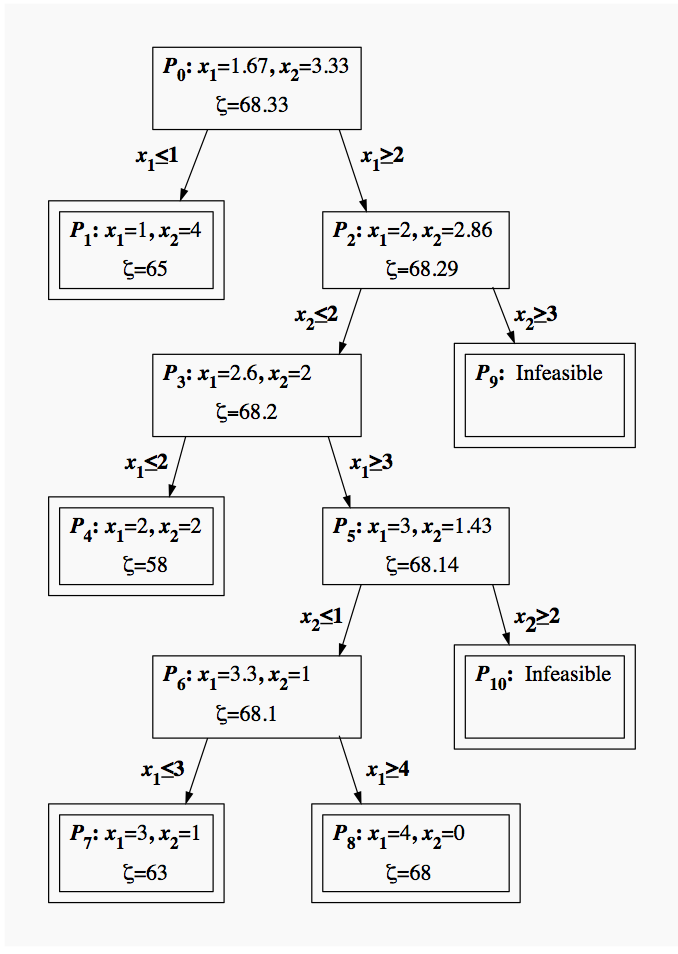
\includegraphics[width=0.6\textwidth]{BNB.png}
    \caption{Enumeration tree that is generated by the branch and bound algorithm for the sample IP problem, taken from
     Linear Programming: Foundations and Extensions by Robert Vanderlei \cite{LPVanderbei}}
\end{figure}

\section{Constraints Programming}
Unlike the programming that we have observed so far, constraints programming (CP) is a programming paradigm that is implemented
in LP solvers \cite{wiki:cp}. It is a programming paradigm that combines declarative and procedural paradigm \cite{wiki:cp, Bockmayr2003}.
This seems contradictory at first, because declarative formulation is static whereas a procedural one is dynamic. The idea is boiled down to viewing
a constraint the same way as invoking a procedure. The goal of CP is to find feasible solutions out of large solutions space, making it
more suitable to accomodate LP. CP focuses on the constraints and variables rather than the objective function.

In this paradigm, a constraint program may be written declaratively but should be viewed as a procedure that operates on a
solution space. Each constraints will be added to a constraint store, which limits the space that must be searched.
Constraint store uses a filtering algorithm that serves as a litmus test for solutions \cite{Bockmayr2003}.
At the end of the filtering procedure, we obtain a feasible solution.

Given this view, constraint programming formulation tends to look
more like a mathematical programming model than a computer program, since the user writes constraints declaratively
rather than writing procedures to enforce these constraints. For this reason, programming environment that adopts CP
is more suited for solving LP based problems in a computer.

\section{Tools}
In this project, we will be using three LP tools: Gurobi\footnote{See \url{http://gurobi.com}},
or-tools\footnote{See \url{https://developers.google.com/optimization/}} and Optaplanner\footnote{See \url{http://www.optaplanner.org}}.
These tools have their own unique APIs and input format. These tools come with their own version of LP solver that
have unique strengths and weaknesses, as we shall observe in chapter 5.

Gurobi is a optimisation tool built for solving LP based problems. Its LP solver is written in C and it comes with
APIs to port many different programming languages including Java, C++, Python and a few others. Gurobi allows you
to build any models for any LP problem, giving users full control to implement any algorithms or heuristics that they
prefer. It claims to be the fastest solver amongst 3 other open source solvers \cite{gurobi:solvers}, none
of which are used in this project. Gurobi is one of the most expensive commercial LP solver in the industry
and its used by many corporations such as FedEx, Netflix and Google. Academic licenses is also available for universities
and its affiliated individuals for free.

or-tools by Google is an optimisation suite for solving various optimisation problems, including VRP. It contains a constraint programming
solver, unified interface for other solvers (e.g Gurobi, GLPK, etc), implemented mostly in C++. Like Gurobi, it also comes with APIs
to support other major programming languages, albeit in less variety. This tool allows to focus on modelling the problem at hand, without worrying
too much about the algorithms and the heuristics, as they have been implemented and packaged with the solver. It is an open souce
software that is used in internally at Google that offers various advantages such as: high quality, portability and active user community.

Optaplanner is an constraint programming engine built in Java for solving optimisation problems. Unlike the other two solvers, it does not
have API to support other languages. In addition, it takes the input in the form of XML file, which are then processed by the engine. It has
predefined XML tags used to model various problems and built-in implementation of algorithms and heuristics for solving them. What Optaplanner
lacks in portability, it makes it up in usability. The XML input format allows users to define the problem rather than implementing the procedures
to solve the problem. In addition to usability, it comes with a GUI that visualise common optimisation problems, including the VRP.

\section{Graph Theory}
In this section we discuss some relevant terminologies \cite{wilson1996} from graph theory to get a better understanding of
the ideas discussed in the vehicle routing problem:
\begin{itemize}
\item A \textbf{graph} is a collection of points connected by lines in a plane. The points and lines are
more commonly refered to as \textbf{vertices} and \textbf{edges} respectively.
\item A \textbf{directed} graph is a graph whose edges goes in one direction but not the other.
\item An \textbf{undirected} graph has edges that goes in both directions.
\item A \textbf{complete} graph where all of its vertices are connected to one another.
\item A \textbf{walk} is a sequence of vertex and edges that connects one vertex to another in a graph.
\item A \textbf{path} is a walk in which no vertex appers more than once. It is also more commonly refered to as a \textbf{hamiltonian path}.
\item A \textbf{cycle} is a walk such that the first vertex corresponds with the last.
\item A \textbf{hamiltonian cycle} is hamiltonian path that also happens to be a cycle.
\end{itemize}

\section{Computational Complexity}
Talk about decision problems and its classifications, P and NP problems and how does it affect the computation of the problem.
We classify easy and hard problems in Computer Science depending on whether they can be solved by an Algorithm within polynomial time or not.
The problems are restricted to decision problems, which are problems that can be answered with a yes or a no. Decision problems fall into
two main important classes: P and NP. P class consists of decision problems in which polynomial time algorithm exists. On the other hand,
NP class consists of decision problems that can be solved by non-deterministic turing machine\footnote{refer to wikipedia} in polynomial time.
Or in other words, it can be determined if this problem has a solution in polynomial time???(must check this again..). Explain NP hard and
NP completeness
Explain the question if P=NP?Lenstra et al \cite{here} explains that VRP is hard. This is because..

This means that we have to use efficient algorithm otherwise it would take too long to compute. Imagine doing a brute force algorithm, it
would take very long time to compute. Linear programming is the best method out there that has polynomial running time... or something like
that... Due to the nature of the problem, it may take very long time to compute it.

\section{Review}
In this chapter, we have introduced the key concepts that are recurring throughout the project. Linear programming is a
mathematical method concerns with finding an optimal value of a function in a linear system under a set of constraints. Integer
programming is linear programming with the additional constraint where all of its decision variables are restricted to integers.
There are several algorihtms to find the optimal value of the objective function in a linear program such as simplex and branch-and-bound
algorithm. We also explained constraints programing, a programming paradigm that helps software engineers implement program
to solve linear programs and some background information on LP tools used in this project. Lastly, we covered some basic
concepts in graph theory that will be mentioned quite frequently throughout the project. In particular, is term hamiltonian cycle, which is
a term used to describe a sequence of vertices in a path where each node is visited only once ending in the first node, thus forming a cycle.
